\documentclass{scrartcl}
\usepackage[utf8]{inputenc}
\usepackage[UKenglish]{babel}
\usepackage{caption}
\usepackage{listings}
\usepackage{pdfpages}
\usepackage{amsmath}

\lstset{frame=single,keepspaces=true,captionpos=b}

\title{Homework 01 - kNN \& Decision Trees}
\author{Arne Sachtler - \textit{Registration Number: 03692662}}
\date{\today}
\subtitle{IN2064 Machine Learning}

\begin{document}
\maketitle
	
\section{Problem 1}
The tree is built automatically by a written python script. It prints the resulting tree by a textual description:
\lstinputlisting[caption={Final decision tree generated from the given exemplary data with a maximum depth of two.}]{tree_text}

Generating a set of artificial test data and using the generated decision tree in order to predict the class of the generated test data reveals the learned class decision as shown in Figure~\ref{fig:tree}.

\begin{figure}[h]
	\centering
	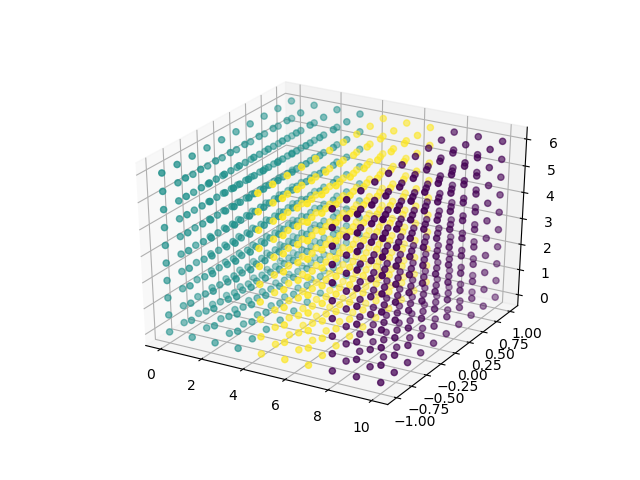
\includegraphics[height=5cm]{figure_tree.png}
	\caption{Class prediction for artificially generated test data.}
	\label{fig:tree}
\end{figure}

\section{Problem 2}
The following table summarises the predicted classes for the two given data points.

\begin{table}[h]
	\centering

	\begin{tabular}{l|c|c}
	\hline

	\hline
	\textbf{Data Point} $\mathbf{x}$ & \textbf{Predicted Class} $y$ & \textbf{Probability} $p(c = y | \mathbf{x}, T)$\\
	\hline
		 $\mathbf{x_a} = \begin{pmatrix}
		 	4.1 & -0.1 & 2.2
		 \end{pmatrix}^\top$& $y_a = 1$ & $p(c = y_a | \mathbf{x}_a, T) = 100\% $\\
	\hline
		$\mathbf{x_b} = \begin{pmatrix}
			6.1 & 0.4 & 1.3
		\end{pmatrix}^\top$ & $y_b = 2$ & $p(c = y_b | \mathbf{x}_b, T) = 66.6\% $\\

	\hline
	\end{tabular}
	\caption{Predicted classes for the given data points by the learned decision tree.}
	\label{tab:class_predictions}
\end{table}

\section{Problem 3}
See the pdf pages attached.

\section{Problem 4}
Using the array function of the numpy library, the $k$NN algorithm can be implemented straightforwardly. The following source code shows the implemented $k$NN implementation.\pagebreak
The predicted class labels for the vectors $\mathbf{x}_a$ and $\mathbf{x}_b$ equal to $2$.

\lstinputlisting[keywordstyle=\color{blue},breaklines=true,caption={Implementation of the $k$NN algorithm.},language=python]{KNN.py}

\begin{table}[h]
	\centering

	\begin{tabular}{l|c}
	\hline

	\hline
	\textbf{Data Point} $\mathbf{x}$ & \textbf{Predicted Class} $y$\\
	\hline
		 $\mathbf{x_a} = \begin{pmatrix}
		 	4.1 & -0.1 & 2.2
		 \end{pmatrix}^\top$& $y_a = 2$\\
	\hline
		$\mathbf{x_b} = \begin{pmatrix}
			6.1 & 0.4 & 1.3
		\end{pmatrix}^\top$ & $y_b = 2$\\

	\hline
	\end{tabular}
	\caption{Predicted classes for the given data points by $k$NN classifier.}
	\label{tab:class_predictions}
\end{table}

\section{Problem 5}
Here the 3-NN classifier is used for regression. Both unweighted and weighted regression are compared. The weighted 3-NN regression uses the euclidean distance in order to determine the weights.

\begin{table}[h]
	\centering

	\begin{tabular}{l|c|c}
	\hline

	\hline
	\textbf{Data Point} $\mathbf{x}$ & \textbf{Unweighted Regression Result} $y$ & \textbf{Weighted Regression Result} $y_w$\\
	\hline
		 $\mathbf{x_a} = \begin{pmatrix}
		 	4.1 & -0.1 & 2.2
		 \end{pmatrix}^\top$& $y_a = 1.0$ & $y_{w,a} = 1.61$\\
	\hline
		$\mathbf{x_b} = \begin{pmatrix}
			6.1 & 0.4 & 1.3
		\end{pmatrix}^\top$ & $y_b = 1.33$ & $y_{w,b} = 1.36$\\

	\hline
	\end{tabular}
	\caption{$k$NN for Regression. Predicted values for unweighted and weighted regression are presented.}
	\label{tab:class_predictions}
\end{table}

\section{Problem 6}
Plotting the dataset reveals the distribution over the space. Figure~\ref{fig:2d} shows scatter plots of the data points as projections onto the three planes spanned by the principal axes. Obviously the feature spaces in the data set are completely different. Different scales and distributions are present. The Euclidean distance is like comparing apples and pears in this example. Another distance metric like the \emph{Mahalanobis} distance promise a better results as this metric explicitly models different variances among different axes. Alternatively, the data can be preprocessed and scales to unit-variance per axis.

As the decision tree algorithm determines the decision threshold and dimensions based on measures like the entropy or the Gini-index, which are independent of the actual values in the feature space, decision trees are robust against different scales in the feature space.


\begin{figure}[h]
	\centering
	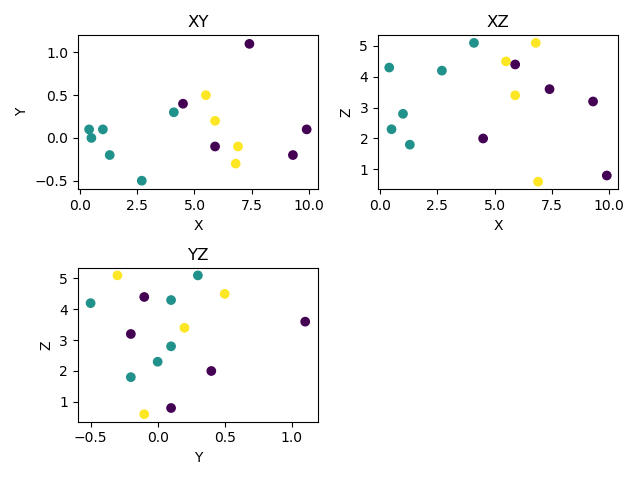
\includegraphics[height=8cm]{2d.png}
	\caption{Plot of the dataset as projections onto the principal planes.}
	\label{fig:2d}
\end{figure}

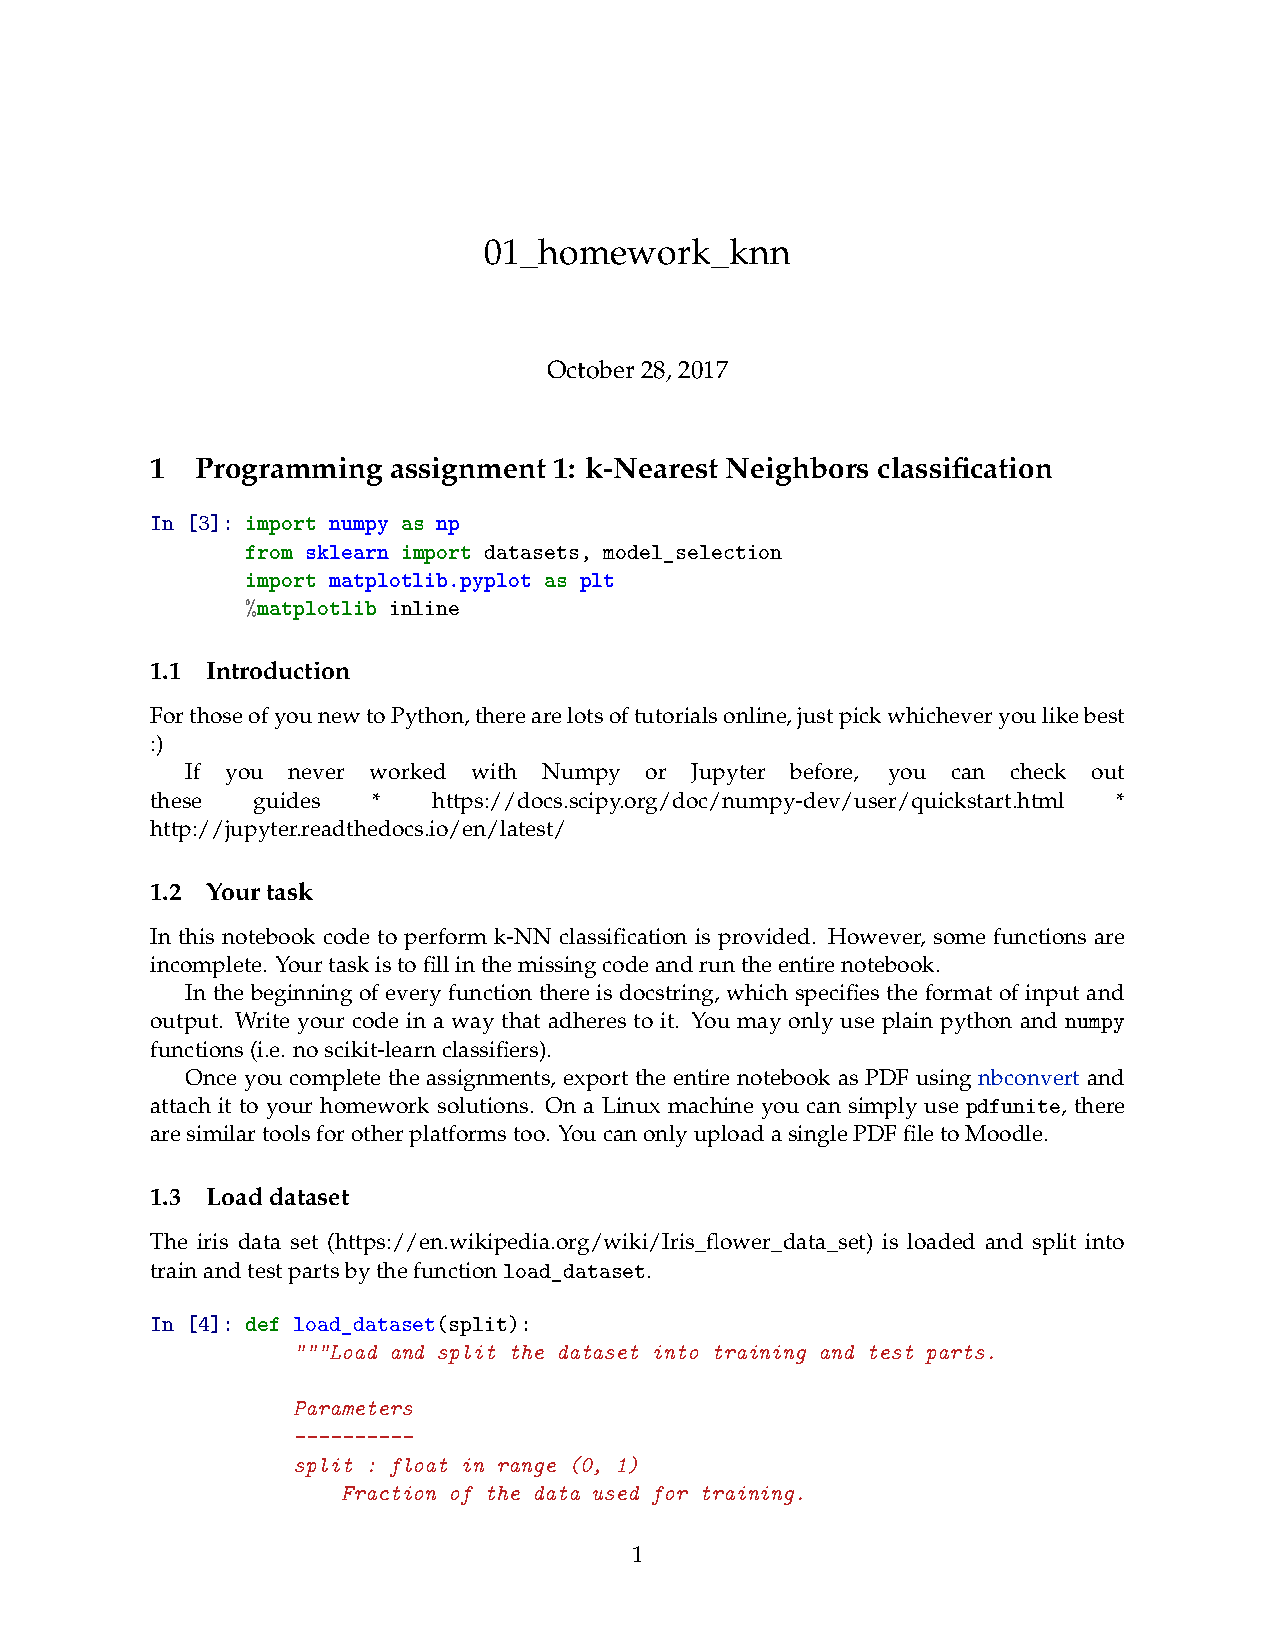
\includepdf[pages=-]{01_homework_knn.pdf}

\end{document}